\documentclass[a4paper,12pt]{article}
\usepackage [left=25.4mm,top=25.4mm]{geometry}
\usepackage{amsmath}
\usepackage{amssymb}
\usepackage{graphicx}
%\usepackage{apacite}
\usepackage{url}
\usepackage{subfig}
\usepackage{csvsimple}
\usepackage{float}
\usepackage{lineno}
\usepackage[affil-it]{authblk}
\usepackage{setspace}
\usepackage{makecell} 
\usepackage{tikz}
\usepackage{csvsimple}
\usepackage{newfloat}
\usepackage{xcolor}
\usepackage{tabularx,booktabs}
\usepackage{multirow}
\usepackage{multicol}
\usepackage{array}
\usepackage{tocbasic}
\usepackage{sectsty}


\begin{document}
	\begin{titlepage}
		\title{Summary of Graph Based Deep Learning Architectures}
		\author{Jarred M. Kvamme}
		\affil{University of Idaho\\ Department of Bioinformatics and Computation Biology}
		\maketitle
	\end{titlepage}
	
	\newpage
	\tableofcontents{}
	\addcontentsline{toc}{section}{LIST OF TABLES}
	\addcontentsline{toc}{section}{LIST OF FIGURES}
	\listoffigures
	\newpage
	\clearpage
	\section{Graph Learning}
	Graph structured data is found in many real-world applications, such as biological networks. Recent advancements in machine learning have allowed neural network models to take advantage of the rich relational information present in graph structured data. Geometric models are generically referred to as graph neural networks (GNNs) in the deep learning paradigm. These models consist of "message-passing" layers - layers which consist of a differentiable aggregation function which iteratively updates node features based on local structure, and then passes the aggregated "message" through dense linear layer and nonlinear activation \cite{scarselli2008graph,gori2005new}. 
	
 	Recently, \cite{kipf2016semi} proposed graph convolutional neural networks (GCNs), as a generalization of convolutional neural networks to graph structured data. GCN performs convolutions on a graph using a 1-step spectral filter which aggregates node and neighbor information together by smoothing node features over a local neighborhood in the graph. However, the learned spectral filters of GCN depend on the eigendecomposition of the spectral graph. Thus the filters are specific to the input graph structure and cannot be directly applied to a graph of with different structure. 
 	
 	Another type of layer is the graph attention network (GAT) \cite{velivckovic2017graph}. GAT integrates Graph Neural Networks (GNNs) with the traditional self-attention mechanism \cite{bahdanau2014neural}. When applied to graph-structured data, the attention coefficients serve as a valuable tool for quantifying the significance of a node's neighbors, enabling the model to prioritize important relationships among nodes.
	\subsection{Generic Graph Neural Networks (GNN)}
	A generic graph neural network consists of message passing layers in which structural information is used to determine which nodes allowed to share feature information based on local linkages. A simple GNN model takes as input an attributed graph $\mathcal{G}(E,V, {\bf X})$ with $V={V_i}_{i=1}^N$ vertices, $e_{i,j} \in E$ edges between vertices, and node attributes ${\bf X}$. The following is the generic architecture of a message-passing layer.
	\begin{eqnarray} {\bf h}_u = \psi\left({\bf x}_u \cdot \underset{v\in\mathbb{N}}{\text{AGGREGATE}}\big(\phi({\bf x}_u, {\bf x}_v), e_{u,v}\big)\right) \label{eq:eqn3}\end{eqnarray}
	where ${\bf h}_u$ is the updated representation of node $u$, ${\bf x}_u$ is the feature vector for node $u$, ${\bf x}_v$ is the feature vector of node $v$, and $e_{u,v} = (u,v)$ is the edge between nodes $u$ and $v$, and $\phi$ and $\psi$ are differentiable activation activation functions.
	\subsection{Graph Convolutional Neural Network (GCN)}
	\cite{kipf2016semi} presented a spectral view of graph convolutions as the 1-D signal Fourier transform in the spectral graph domain \cite{zhang2019graph}. In the GCN architecture, the graph structure is encoded by the normalized Laplacian ${\bf \tilde L}$ representation of the adjacency matrix ${\bf A}$.
	
	\[ H = \phi\left({\bf \tilde LXW}\right) \]  
	
	where ${\bf \tilde L}$ is the normalized graph Laplacian with added self loops such that ${\bf \tilde L} = {\bf D}^{1/2}{\bf I + A}{\bf D}^{1/2}$ 
	
	\subsection{Graph Attention Neural Network (GAT)}
	The GAT model is similar to GNN/GCN in that the contribution of source nodes to a given target is a weighted average. However, in the GAT model, the weight applied to each node is a function of the source and targets nodes embeddings. This differs from classical GNN/GCN in which the weights are the node degrees. This additional flexibility allows GAT to capture more complex relationships between nodes such as their features or local structure. The GAT layer is defined as 
	\[ \]
	
	
	\section{Geometric Autoencoder Architectures}
	Autoencoders are generative models which consist of two main components (i) an encoder which learns a lower dimension representation of the data which are embedded at a bottleneck layer and (ii) a decoder which reconstructs the embeddings back to their original input. In geometric learning, the autoencoder framework has been routinely employed for a number of deep learning task including community detection \cite{kipf2016variational,wang2017mgae,zhou2023community,wang2021scgnn}. However, these methods are typically restricted to reconstructing either the graph or the node attributes but rarely both.  
	\subsection{Graph AutoEncoder (GAE)}
	GAE is the non-probabilistic version of the variational autoencoder first proposed by \cite{kipf2016variational} for node classification. GAE takes as input an attributed graph and passes the graph and node-features through two GCN encoder layers which learn a representation $\bf Z$ which can be used to do a number of tasks. The "decoder" of GAE consists of a simple non-trainable layer they call the "dot-product decoder" as it takes the outer product of $\bf Z$ followed by logistic activation to reconstruct the input graph.  The encoder layers are given by 
	\[ h_u =  ReLU\left(\sqrt{\frac{1}{d_u}}\sum_{v\in \mathcal{N}(u)}^n \sqrt{\frac{1}{d_v}} {\bf W}h_v\right)\]
	
	The decoder layer is given as
	
	\[ \hat{\bf A} = \sigma({\bf ZZ}^T) \]
	\begin{figure}[H]
		\centering
		\caption{Graph AutoEncoder (GAE) Architecture}
		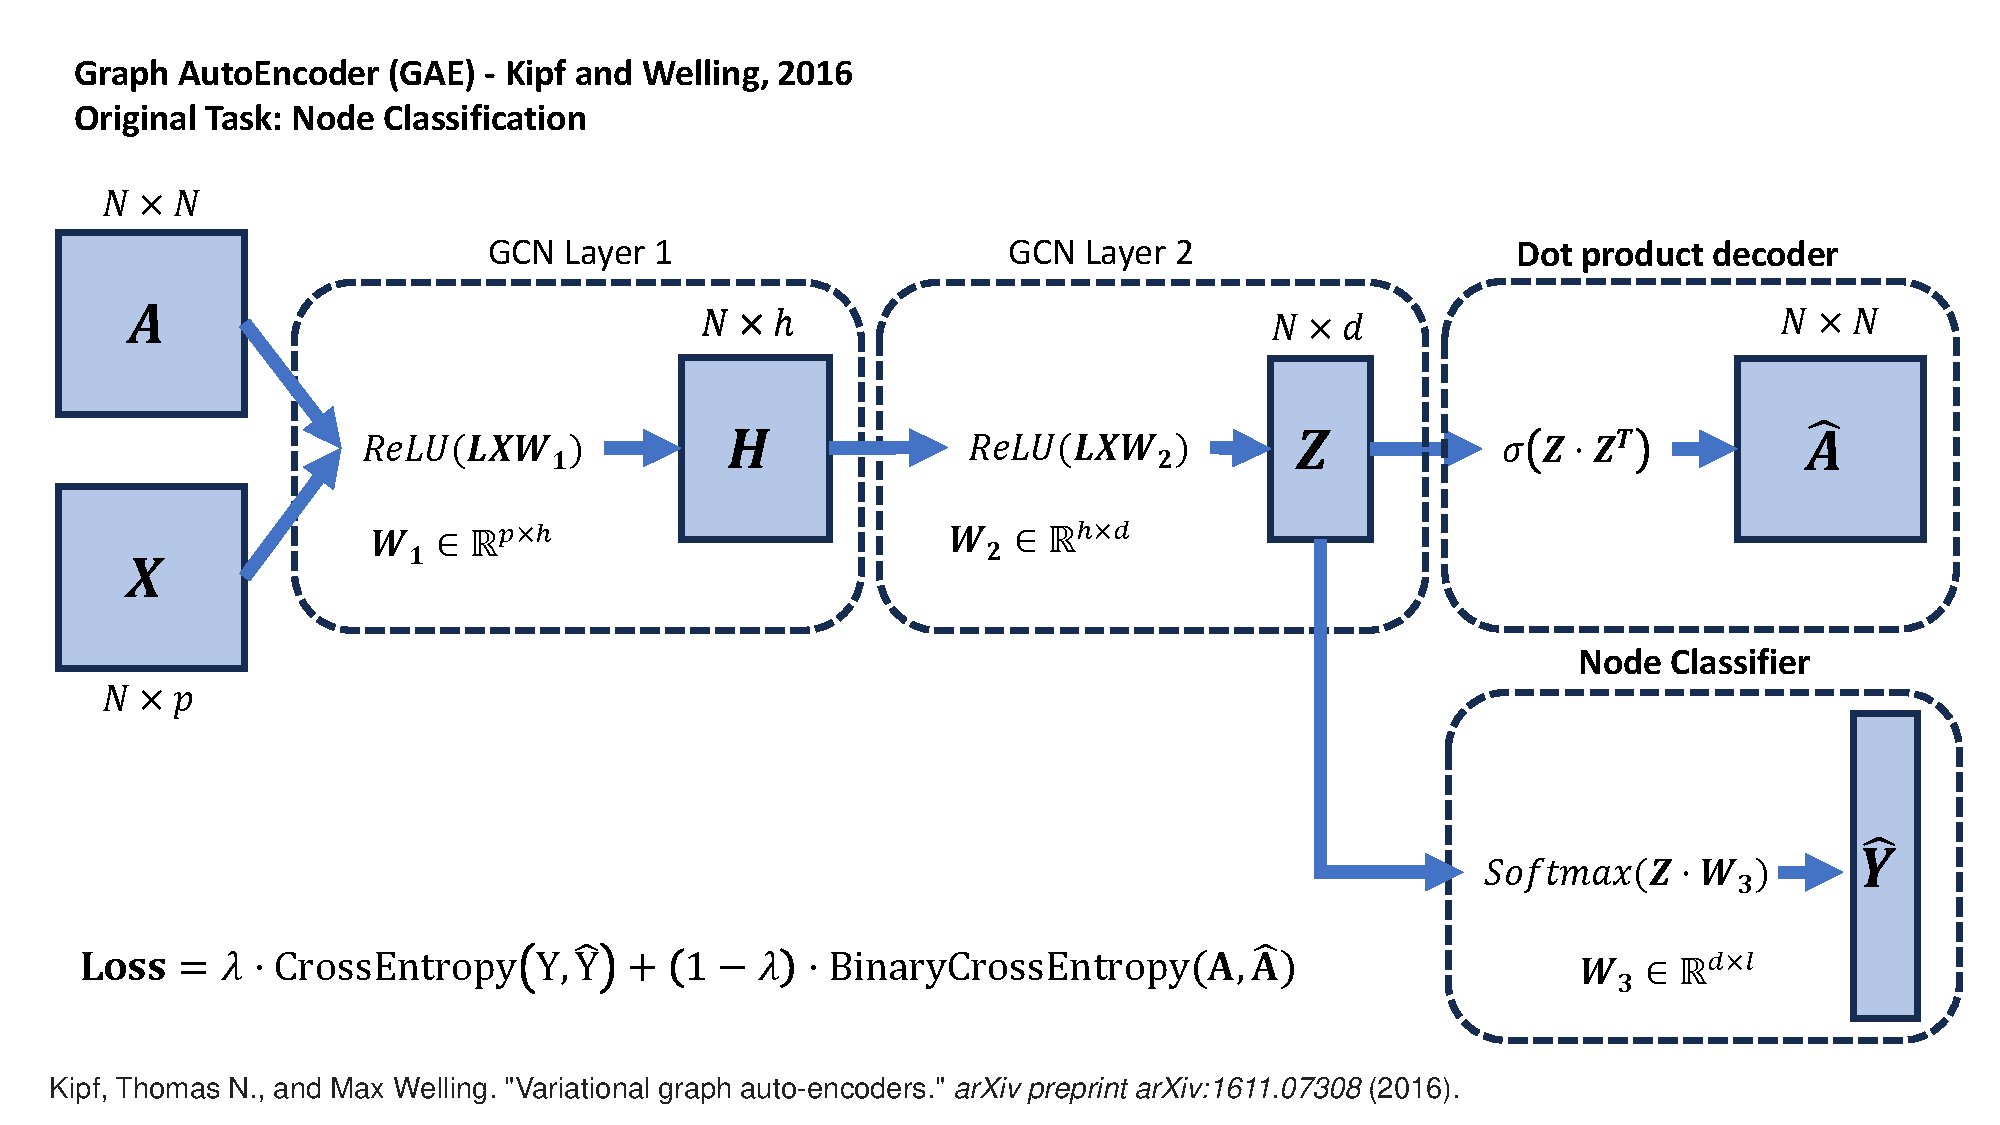
\includegraphics[scale=0.5]{C:/Users/Bruin/Documents/GitHub/HGRN_repo/HGRN_pseudocode/GAE_architecture.pdf}
		\label{fig:gae_mod}
	\end{figure}
	
	
	
	\subsection{Graph Attention Autoencoder (GATE)}
	The authors \cite{salehi2019graph} propose graph attention autoencoder (GATE) which uses conventional GAT layers in an autoencoder framework to reconstruct both the node attributes and graph structure for both supervised and unsupervised graph learning tasks \textbf{Figure \ref{fig:gate}} for node classification and link prediction. The reconstructed node attributes are taken as the last layer of the decoder model and the reconstructed graph is found using dot-product decoder used in GAE. The attention mechanism is computed as follows
	
	\[ \alpha_{ij} = \frac{\sigma\left(\exp\left({\bf a}_s^T\phi\left[{\bf W}h_i\right]+{\bf a}_v^T\phi\left[{\bf W}h_j \right]\right)\right)}
	{\sum_{k\in \mathcal{N}(i)}\sigma\left(\exp\left({\bf a}_s^T\phi\left[{\bf W}h_i\right]+{\bf a}_v^T\phi\left[{\bf W}h_k \right]\right)\right)} \]
	
	where ${\bf W},{\bf a}_s^T$, and ${\bf a}_v^T$ are learnable parameters, $\phi$ denotes an activation function, and $\sigma$ denotes the logistic sigmoid function. In the original work of \cite{velivckovic2017graph} $\phi$ was given as the LeakyReLU activation. The attention mechanism adopted by \cite{salehi2019graph} is a slight variation of the original self-attention proposed \cite{velivckovic2017graph} which uses separate attention weights for nodes $i$ and $j$ 
	
	\begin{figure}[H]
		\centering
		\caption{Graph Attention Autoencoder (GATE) Architecture}
		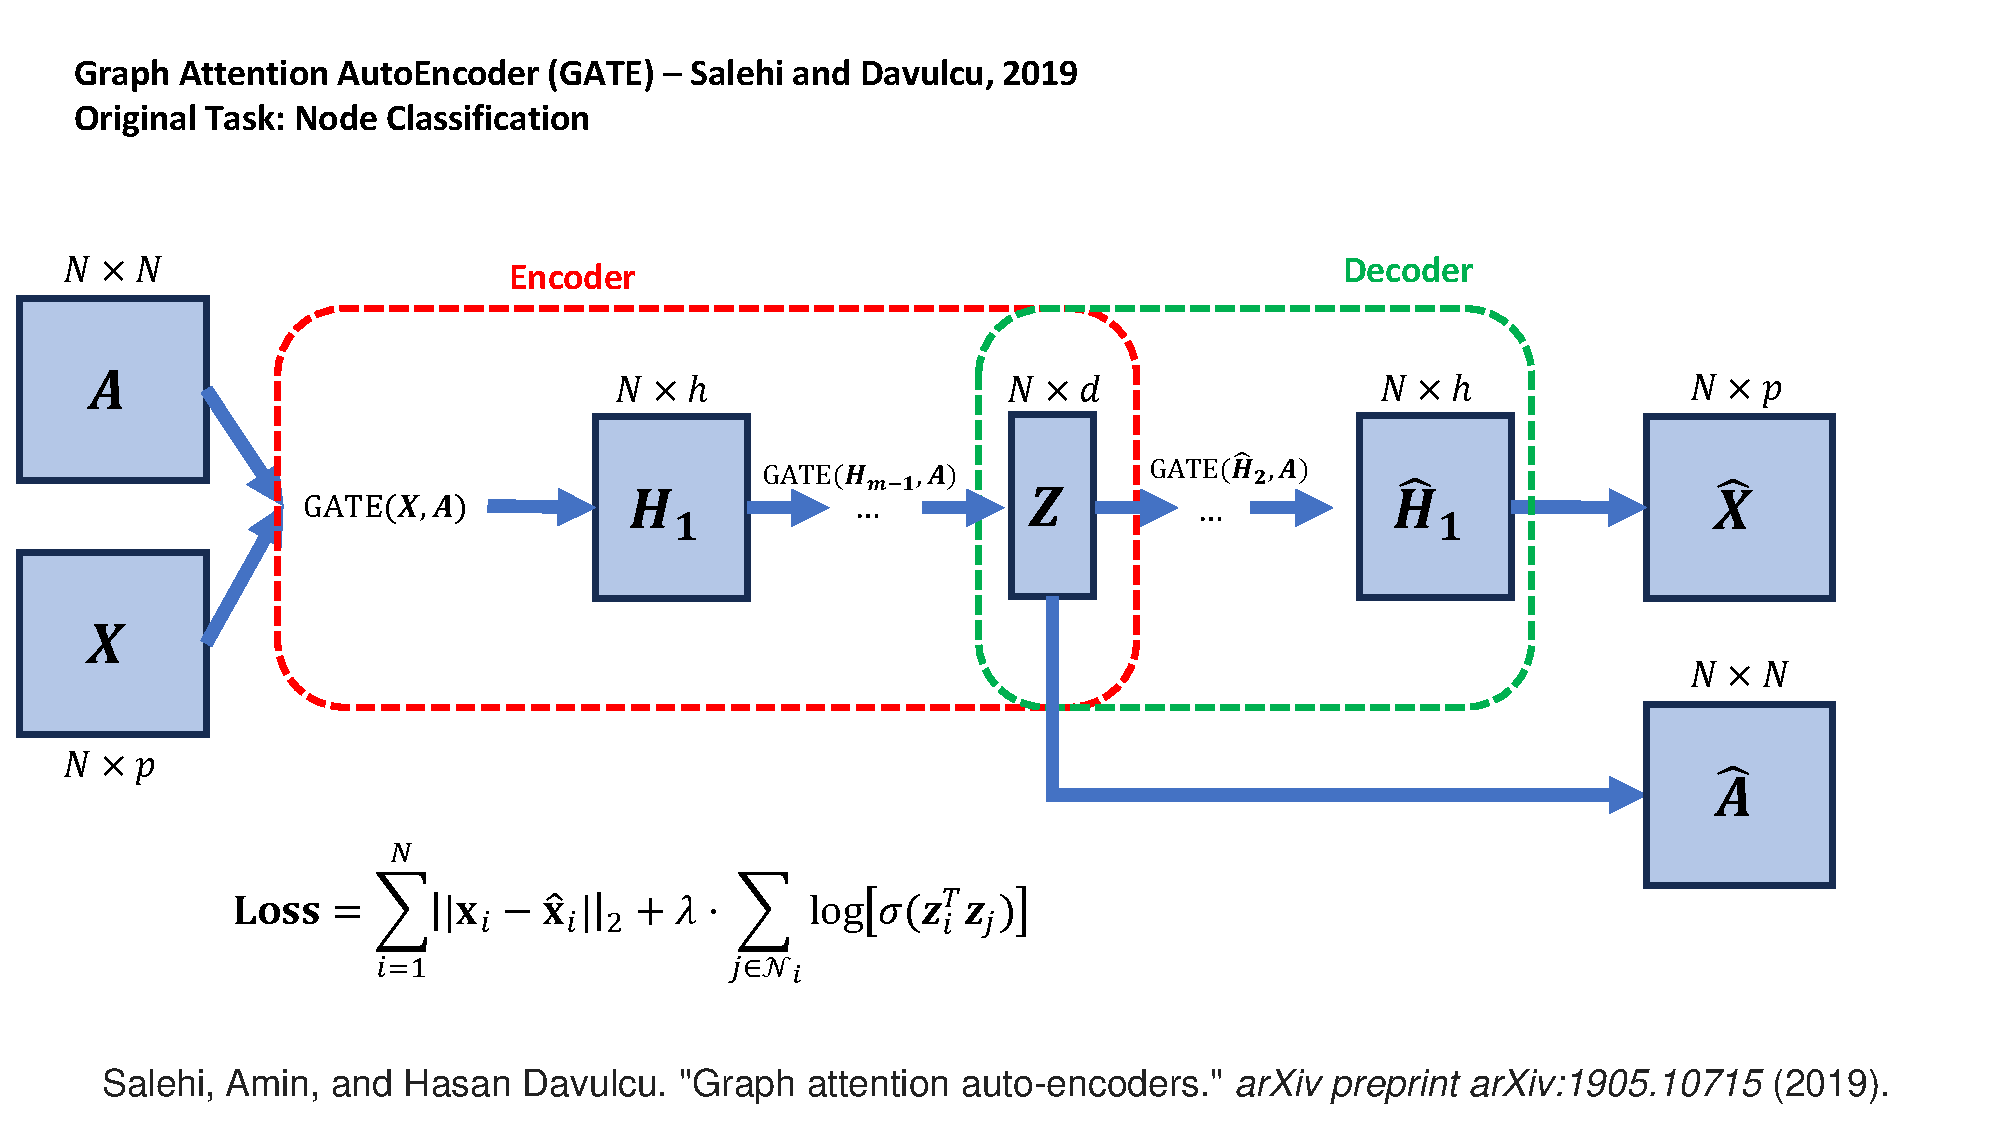
\includegraphics[scale=0.5]{C:/Users/Bruin/Documents/GitHub/HGRN_repo/HGRN_pseudocode/GATE architecture.pdf}
		\label{fig:gate}
	\end{figure}
	
	
	\subsection{Community Detection Based on Unsupervised Attributed Network Embedding (CDBNE)}
	
	CDBNE is a model proposed by \cite{zhou2023community} which adopts GATE under a different loss function for community detection on graphs. Specifically, the CDBNE uses three loss components: (i) A modularity loss $L_M$computed as the modularity of inferred graph communities, (ii) the reconstruction loss $L_R$ which consists of the reconstruction of the node attributes $L_X$ and the reconstruction of the adjacency matrix $L_A$ (iii) a clustering loss $L_C$ based on the KL divergence between the inferred communities and some set of "soft" initial predictions of the communities. The final objective function
	\[ L_{\text{total}} = L_R+\delta L_C-\gamma L_M \]
	which has two tuning parameters $\delta$ and $\gamma$.
	\begin{figure}[H]
		\centering
		\caption{CDBNE Architecture}
		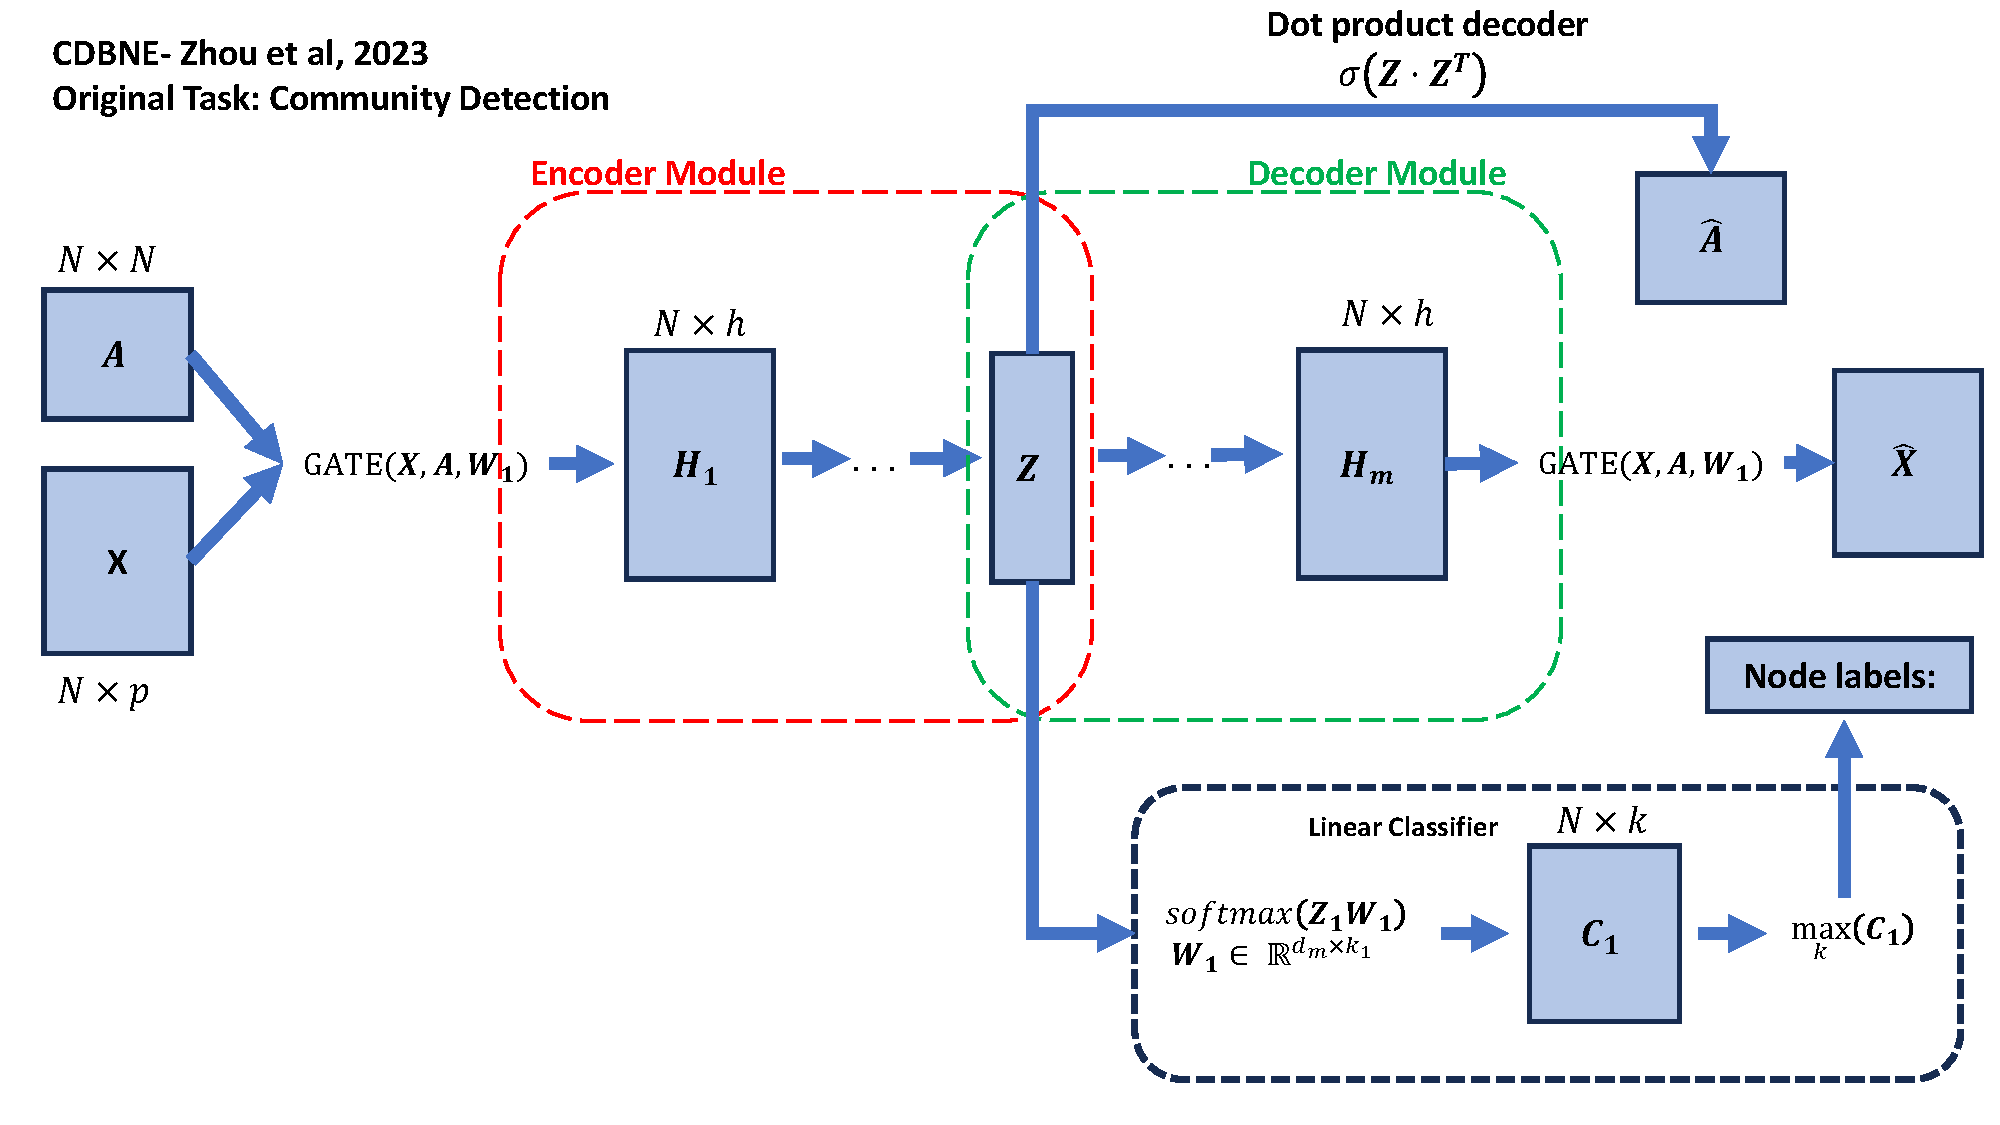
\includegraphics[scale=0.5]{C:/Users/Bruin/Documents/GitHub/HGRN_repo/HGRN_pseudocode/CDBNE_architecture.pdf}
		\label{fig:gae}
	\end{figure}
	
	
	
	
	\section{Metrics for detecting community structure}
	A classical 
	
	
	
	
	
	
	
	
	
	
	
	
	
	
	
	
	
	
	
	
	
	
	
	
	
	
	
	
	
	
	
	
	
	
	
	
	
	
	
	
	
	
	
	
	
	
	
	
	
	
	
	
	
	
	
	
	
	
	
	
	
	
	
	
	
	
	
	
	
	
	
	
	
	
	
	
	
	
	
	
	
	
	\bibliographystyle{unsrt}
	\bibliography{pseudocode_bibs}
	
	
\end{document}